\chapter{การแปลงปริภูมิสีหลากมิติและตารางสอบเทียบมาตรฐานสากล}
\label{ch:multi_color_space}

\section{บทนำและรากฐานทางคณิตศาสตร์ของปริภูมิสีดิจิทัล}

ในการพัฒนาระบบคอมพิวเตอร์วิทัศน์เพื่อการวิเคราะห์คุณสมบัติดิน การพึ่งพาปริภูมิสีแดง เขียว น้ำเงิน (sRGB) เพียงอย่างเดียว ก่อให้เกิดความเปราะบางอย่างมีนัยสำคัญ เนื่องจากความเข้มแสงและการกระเจิงของรังสีตกกระทบส่งผลให้ค่าองค์ประกอบ $R, G, B$ แปรผันตามกันไปในทิศทางเดียวกันทั้งหมด (High Cross-Channel Covariance) ทำให้ยากต่อการแยกแยะระหว่างการเปลี่ยนแปลงทางเคมีสีจริงกับการเปลี่ยนแปลงของระดับความสว่าง เพื่อแก้ปัญหาดังกล่าว สถาปัตยกรรมระบบในคู่มือฉบับนี้จึงนำเสนอการแปลงข้อมูลสีข้าม 4 ปริภูมิสีหลัก ได้แก่ RGB, HSV, CIE $L^*a^*b^*$ และ YCbCr เพื่อสกัดคุณลักษณะเด่นที่มีความเสถียรสูงสุด

\section{ทฤษฎีและสมการการแปลงปริภูมิสี}

\subsection{ปริภูมิสีทรงกระบอก HSV (Hue--Saturation--Value)}
การแปลงพิกัดสีจากระบบ $\text{sRGB}$ ที่ถูกปรับสเกลให้อยู่ในช่วง $[0, 1]$ ไปสู่ปริภูมิสีทรงกระบอก $\text{HSV}$ มีวัตถุประสงค์เพื่อแยกแยะมุมสีแท้ (Hue, $H$) และความอิ่มตัวของสี (Saturation, $S$) ออกจากค่าความสว่าง (Value, $V$) การคำนวณทางคณิตศาสตร์นิยามดังนี้

\begin{equation}
C_{\max} = \max(R, G, B), \quad C_{\min} = \min(R, G, B), \quad \Delta = C_{\max} - C_{\min}
\end{equation}

มุมสีแท้ $H$ คำนวณตามเงื่อนไขของระนาบสีสูงสุด

\begin{equation}
H = \begin{cases} 
0^\circ & \text{ถ้า } \Delta = 0 \\
60^\circ \times \left( \dfrac{G - B}{\Delta} \bmod 6 \right) & \text{ถ้า } C_{\max} = R \\
60^\circ \times \left( \dfrac{B - R}{\Delta} + 2 \right) & \text{ถ้า } C_{\max} = G \\
60^\circ \times \left( \dfrac{R - G}{\Delta} + 4 \right) & \text{ถ้า } C_{\max} = B
\end{cases}
\end{equation}

ความอิ่มตัวของสี $S$ และค่าความสว่าง $V$ นิยามโดย

\begin{equation}
S = \begin{cases} 0 & \text{ถ้า } C_{\max} = 0 \\ \dfrac{\Delta}{C_{\max}} & \text{ถ้า } C_{\max} > 0 \end{cases}, \qquad V = C_{\max}
\end{equation}

สำหรับตัวอย่างสารละลายดิน มุมสีแท้ $H$ จะตอบสนองอย่างไวต่อการเปลี่ยนสถานะของอินดิเคเตอร์วัดกรดด่าง ในขณะที่ค่า $V$ สะท้อนถึงความขุ่นและความสว่างของเม็ดดิน

\subsection{ปริภูมิสีสมมาตรสายตามนุษย์ CIE $L^*a^*b^*$}
ปริภูมิสี $\text{CIE } L^*a^*b^*$ (1976) เป็นปริภูมิสีที่ถูกออกแบบให้มีความสม่ำเสมอเชิงการรับรู้ (Perceptually Uniform Color Space) โดยระยะห่างแบบยุคลิดระหว่างสองจุดสีจะสอดคล้องกับความแตกต่างที่สายตามนุษย์สัมผัสได้จริง การแปลงเริ่มต้นจากการปรับเชิงเส้นของสัญญาณสี $\text{sRGB}$ สู่ระบบ $\text{CIE } XYZ$ ภายใต้สารให้แสงมาตรฐานสากล $\text{D65}$ มุมมองมาตรฐาน 2 องศา จุดขาวอ้างอิง $(X_n, Y_n, Z_n) = (95.047, 100.000, 108.883)$ ดังนี้

\begin{equation}
\begin{bmatrix} X \\ Y \\ Z \end{bmatrix} = \begin{bmatrix} 
0.4124564 & 0.3575761 & 0.1804375 \\
0.2126729 & 0.7151522 & 0.0721750 \\
0.0193339 & 0.1191920 & 0.9503041
\end{bmatrix} \begin{bmatrix} f_{\text{gamma}}(R) \\ f_{\text{gamma}}(G) \\ f_{\text{gamma}}(B) \end{bmatrix}
\end{equation}

โดยฟังก์ชันแก้ไขแกมมาแบบผกผัน (Inverse sRGB Companding) กำหนดดังสมการ

\begin{equation}
f_{\text{gamma}}(C) = \begin{cases} 
\dfrac{C}{12.92} & \text{ถ้า } C \le 0.04045 \\[6pt]
\left( \dfrac{C + 0.055}{1.055} \right)^{2.4} & \text{ถ้า } C > 0.04045 
\end{cases}
\end{equation}

จากนั้นนำค่าพิกัดไตรสติมูลัสสัมพัทธ์เข้าสู่ฟังก์ชันไม่เชิงเส้นลูกบาศก์รูท

\begin{equation}
f(t) = \begin{cases}
t^{1/3} & \text{ถ้า } t > \delta^3 \\[6pt]
\dfrac{t}{3 \delta^2} + \dfrac{4}{29} & \text{ถ้า } t \le \delta^3
\end{cases}
\end{equation}

โดยที่ $\delta = 6/29$ นำไปสู่การคำนวณค่า $L^*, a^*, b^*$ ดังสมการ

\begin{align}
L^* &= 116 \cdot f\left( \frac{Y}{Y_n} \right) - 16 \\
a^* &= 500 \cdot \left[ f\left( \frac{X}{X_n} \right) - f\left( \frac{Y}{Y_n} \right) \right] \\
b^* &= 200 \cdot \left[ f\left( \frac{Y}{Y_n} \right) - f\left( \frac{Z}{Z_n} \right) \right]
\end{align}

แกน $a^*$ บ่งบอกทิศทางจากสีเขียว (ค่าลบ) สู่สีแดงอมม่วง (ค่าบวก) ซึ่งสัมพันธ์กับปฏิกิริยาสีย้อมเอโซของไนโตรเจน ในขณะที่แกน $b^*$ บ่งบอกทิศทางจากสีน้ำเงิน (ค่าลบ) สู่สีเหลือง (ค่าบวก) ซึ่งสัมพันธ์อย่างยิ่งกับปฏิกิริยาโมลิบดินัมบลูของฟอสฟอรัส

\subsection{ปริภูมิสีแยกสัญญาณความสว่าง YCbCr}
ตามมาตรฐานสากล $\text{ITU-R BT.601}$ การแยกสัญญาณความสว่าง ($Y$) ออกจากสัญญาณความต่างสีน้ำเงิน ($C_b$) และสัญญาณความต่างสีแดง ($C_r$) ช่วยเพิ่มความแม่นยำในการตรวจวัดเมื่อตัวอย่างดินมีความชื้นสูง

\begin{align}
Y &= 0.299 \cdot R + 0.587 \cdot G + 0.114 \cdot B \\
C_b &= 128 - 0.168736 \cdot R - 0.331264 \cdot G + 0.5 \cdot B \\
C_r &= 128 + 0.5 \cdot R - 0.418688 \cdot G - 0.081312 \cdot B
\end{align}

\section{การสร้างเวกเตอร์คุณลักษณะสี 9 มิติเพื่อป้อนสู่โมเดล}

จากการสกัดค่าเฉลี่ยเชิงพื้นที่ในบริเวณที่ผู้ใช้เลือกวิเคราะห์ (Region of Interest, ROI) ระบบจะสร้างเวกเตอร์คุณลักษณะสีรวม 9 มิติดังนี้

\begin{equation}
\mathbf{x}_{\text{color}} = \left[ R_{\text{norm}}, \, G_{\text{norm}}, \, B_{\text{norm}}, \, \frac{H}{360}, \, S, \, V, \, \frac{L^*}{100}, \, \frac{a^* + 128}{255}, \, \frac{b^* + 128}{255} \right]^T \in \mathbb{R}^9
\end{equation}

เวกเตอร์ดังกล่าวผ่านการปรับมาตรฐานให้อยู่ในช่วง $[0, 1]$ อย่างสมบูรณ์ เพื่อป้องกันไม่ให้ค่าน้ำหนักของโครงข่ายประสาทเทียมเอียงเอนไปยังตัวแปรที่มีขนาดตัวเลขสูงกว่า

\section{ตารางสอบเทียบมาตรฐานสากลของคุณสมบัติดิน}

คณะผู้วิจัยได้ดำเนินการสร้างชุดข้อมูลอ้างอิงเชิงมาตรวิทยา โดยใช้สารละลายบัฟเฟอร์มาตรฐานที่ผ่านการรับรองตามมาตรฐาน $\text{NIST Traceable}$ ร่วมกับชุดทดสอบเคมีมาตรฐานสากล ได้ผลลัพธ์พิกัดสีมาตรฐานสำหรับการสอบเทียบดังแสดงในตารางที่ \ref{tab:ph_standards} และตารางที่ \ref{tab:npk_standards}

\begin{table}[H]
\centering
\caption{พิกัดสีมาตรฐานสำหรับการสอบเทียบระดับความเป็นกรดด่างของสารละลายดิน}
\label{tab:ph_standards}
\small
\begin{tabularx}{\textwidth}{c c c c c c}
\toprule
\textbf{ระดับ pH} & \textbf{สถานะดิน} & \textbf{รหัสฐานสิบหก} & \textbf{RGB} & \textbf{HSV (องศา, \%, \%)} & \textbf{CIE $L^*a^*b^*$} \\
\midrule
4.0 & กรดรุนแรงมาก & \texttt{\#D32F2F} & (211, 47, 47) & (0, 78, 83) & (46.2, 63.8, 41.5) \\
5.0 & กรดปานกลาง & \texttt{\#FF9800} & (255, 152, 0) & (36, 100, 100) & (69.8, 32.1, 74.5) \\
6.0 & กรดเล็กน้อย & \texttt{\#FDD835} & (253, 216, 53) & (49, 79, 99) & (87.1, 0.4, 78.6) \\
6.5 & เหมาะสมต่อพืช & \texttt{\#8BC34A} & (139, 195, 74) & (88, 62, 76) & (73.5, -34.8, 52.4) \\
7.0 & เป็นกลาง & \texttt{\#4CAF50} & (76, 175, 80) & (122, 57, 69) & (64.2, -45.1, 38.6) \\
7.5 & ด่างเล็กน้อย & \texttt{\#009688} & (0, 150, 136) & (174, 100, 59) & (56.4, -36.2, -1.2) \\
8.5 & ด่างรุนแรง & \texttt{\#3F51B5} & (63, 81, 181) & (231, 65, 71) & (38.8, 25.1, -55.8) \\
\bottomrule
\end{tabularx}
\end{table}

\begin{table}[H]
\centering
\caption{ระดับความเข้มข้นและพิกัดสีมาตรฐานสำหรับการวิเคราะห์ธาตุอาหารหลัก N-P-K}
\label{tab:npk_standards}
\small
\begin{tabularx}{\textwidth}{c c c c c}
\toprule
\textbf{ธาตุอาหาร} & \textbf{ระดับประเมิน} & \textbf{ช่วงความเข้มข้น} & \textbf{รหัสสีอ้างอิง} & \textbf{RGB อ้างอิง} \\
\midrule
ไนโตรเจน (N) & ต่ำมาก (Very Low) & $< 15\text{ mg/kg}$ & \texttt{\#FFE0B2} & (255, 224, 178) \\
& ต่ำ (Low) & $15 - 30\text{ mg/kg}$ & \texttt{\#FFB74D} & (255, 183, 77) \\
& ปานกลาง (Medium) & $30 - 60\text{ mg/kg}$ & \texttt{\#FF7043} & (255, 112, 67) \\
& สูง (High) & $60 - 90\text{ mg/kg}$ & \texttt{\#E64A19} & (230, 74, 25) \\
& สูงมาก (Very High) & $> 90\text{ mg/kg}$ & \texttt{\#BF360C} & (191, 54, 12) \\
\midrule
ฟอสฟอรัส (P) & ต่ำมาก (Very Low) & $< 5\text{ mg/kg}$ & \texttt{\#E1F5FE} & (225, 245, 254) \\
& ต่ำ (Low) & $5 - 15\text{ mg/kg}$ & \texttt{\#81D4FA} & (129, 212, 250) \\
& ปานกลาง (Medium) & $15 - 30\text{ mg/kg}$ & \texttt{\#29B6F6} & (41, 182, 246) \\
& สูง (High) & $30 - 50\text{ mg/kg}$ & \texttt{\#0288D1} & (2, 136, 209) \\
& สูงมาก (Very High) & $> 50\text{ mg/kg}$ & \texttt{\#01579B} & (1, 87, 155) \\
\midrule
โพแทสเซียม (K) & ต่ำมาก (Very Low) & $< 40\text{ mg/kg}$ & \texttt{\#FFF9C4} & (255, 249, 196) \\
& ต่ำ (Low) & $40 - 80\text{ mg/kg}$ & \texttt{\#FFF176} & (255, 241, 118) \\
& ปานกลาง (Medium) & $80 - 150\text{ mg/kg}$ & \texttt{\#FFD54F} & (255, 213, 79) \\
& สูง (High) & $150 - 250\text{ mg/kg}$ & \texttt{\#FFA000} & (255, 160, 0) \\
& สูงมาก (Very High) & $> 250\text{ mg/kg}$ & \texttt{\#FF6F00} & (255, 111, 0) \\
\bottomrule
\end{tabularx}
\end{table}

\begin{figure}[H]
\centering
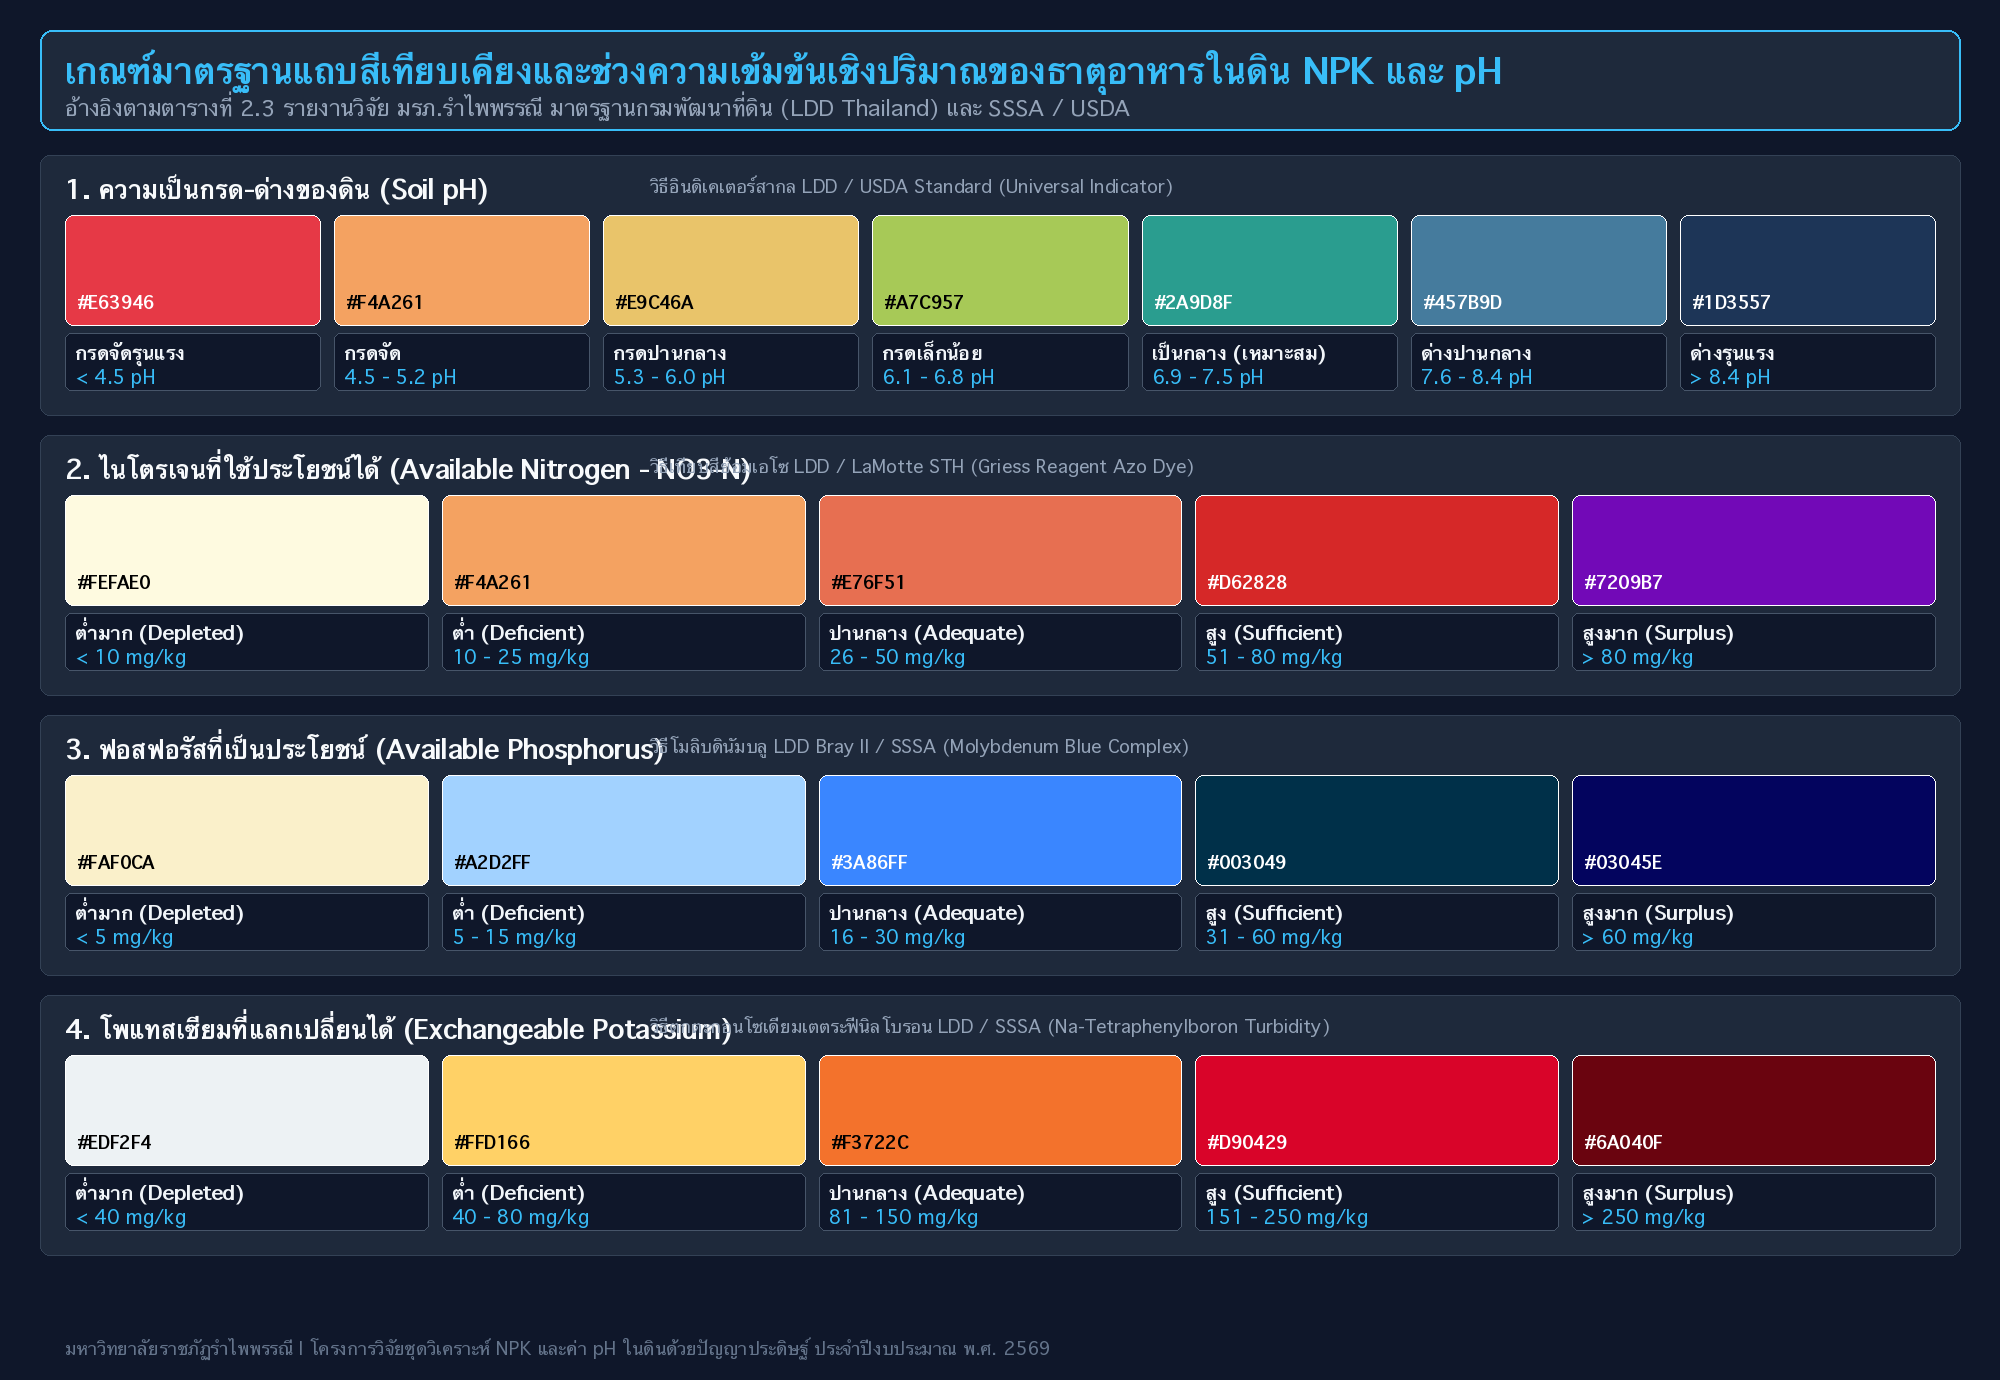
\includegraphics[width=0.88\textwidth]{figures/fig_standard_color_matrix_ch02.png}
\caption{เมทริกซ์การกระจายตัวของพิกัดสีมาตรฐาน 4 ปริภูมิสีสำหรับชุดตรวจสารละลายดิน}
\label{fig:color_matrix_ch02}
\end{figure}

\begin{figure}[H]
\centering
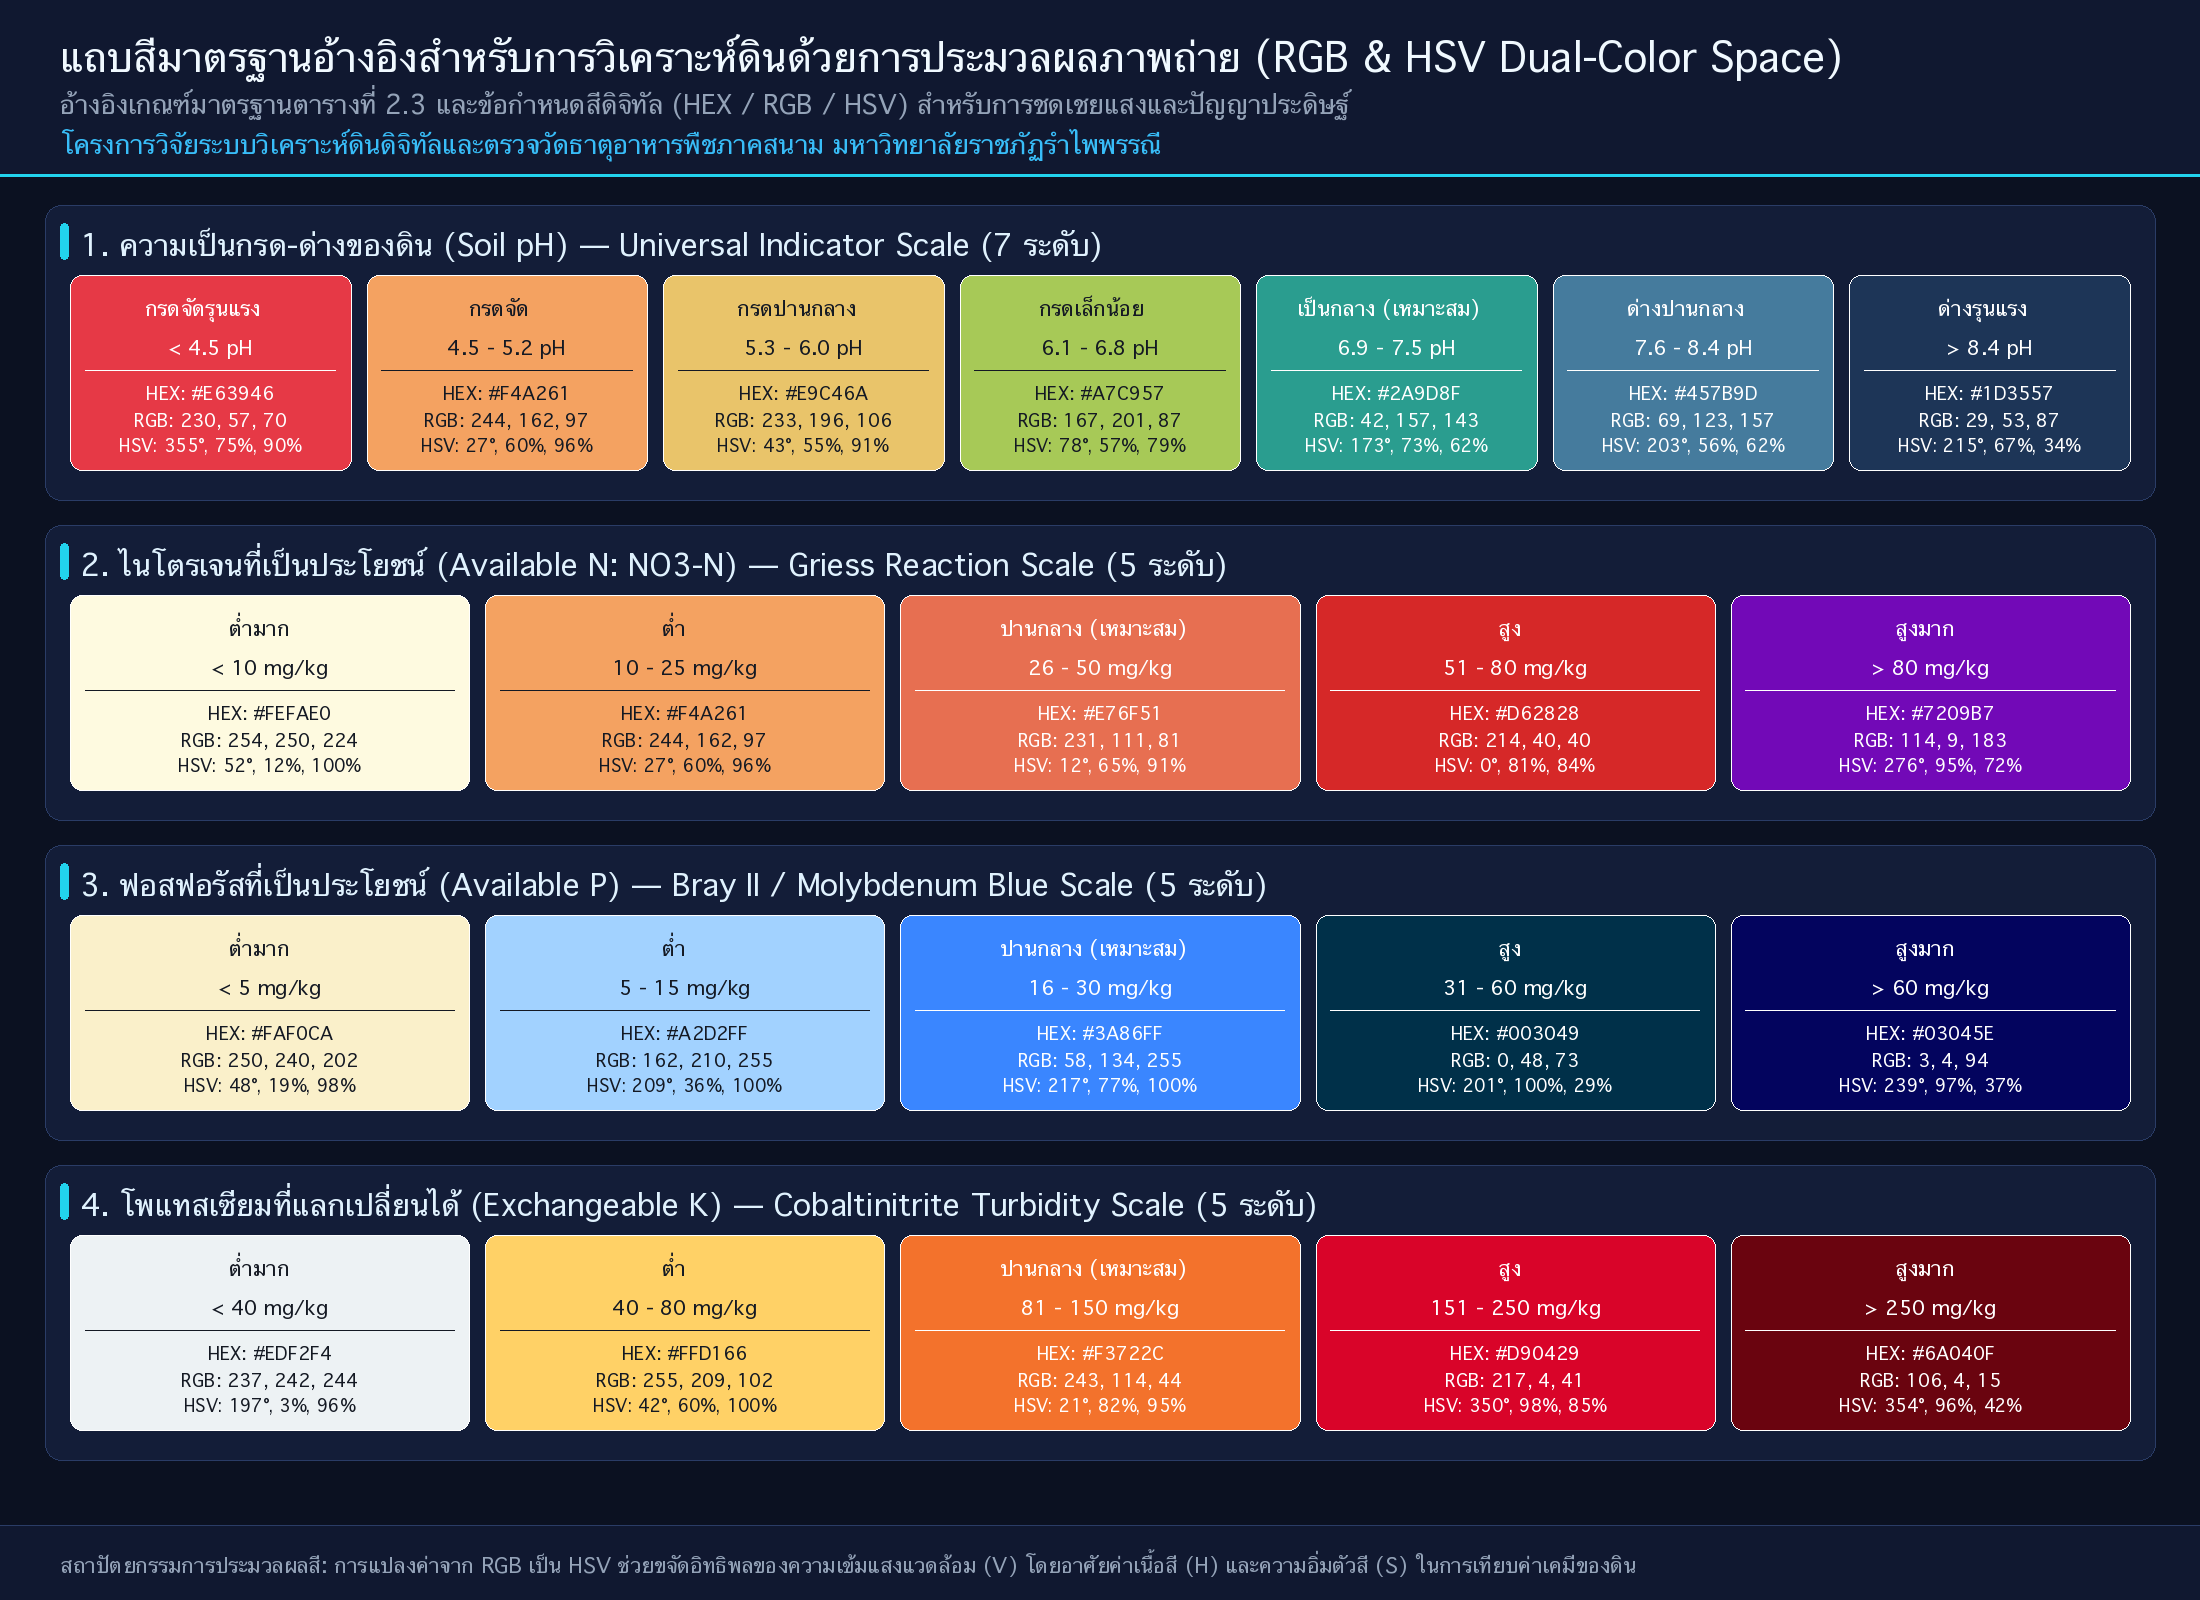
\includegraphics[width=0.88\textwidth]{figures/fig_standard_color_matrix_rgb_hsv.png}
\caption{ระนาบความสัมพันธ์ระหว่างค่ามุมสีแท้ HSV และสภาพสะท้อนแสงจำเพาะในระบบ RGB}
\label{fig:color_matrix_rgb_hsv}
\end{figure}

การเปรียบเทียบพิกัดสีในภาพที่ \ref{fig:color_matrix_ch02} และภาพที่ \ref{fig:color_matrix_rgb_hsv} ยืนยันว่าการใช้คุณลักษณะร่วมข้ามปริภูมิสีทำให้เกิดระนาบการจำแนกเชิงเส้นและไม่เชิงเส้นที่ชัดเจน ป้องกันการทับซ้อนกันของข้อมูลแม้ในกรณีที่สารละลายมีความขุ่นสูง
